% This is samplepaper.tex, a sample chapter demonstrating the
% LLNCS macro package for Springer Computer Science proceedings;
% Version 2.20 of 2017/10/04
%
\documentclass[runningheads]{llncs}
%
\usepackage{graphicx}
\graphicspath{ {./img/} }

% Copyright 2017 Sergei Tikhomirov, MIT License
% https://github.com/s-tikhomirov/solidity-latex-highlighting/

\usepackage{listings, xcolor}

\definecolor{verylightgray}{rgb}{.97,.97,.97}

\lstdefinelanguage{Solidity}{
	keywords=[1]{anonymous, assembly, assert, balance, break, call, callcode, case, catch, class, constant, continue, constructor, contract, debugger, default, delegatecall, delete, do, else, emit, event, experimental, export, external, false, finally, for, function, gas, if, implements, import, in, indexed, instanceof, interface, internal, is, length, library, log0, log1, log2, log3, log4, memory, modifier, new, payable, pragma, private, protected, public, pure, push, require, return, returns, revert, selfdestruct, send, solidity, storage, struct, suicide, super, switch, then, this, throw, transfer, true, try, typeof, using, value, view, while, with, addmod, ecrecover, keccak256, mulmod, ripemd160, sha256, sha3}, % generic keywords including crypto operations
	keywordstyle=[1]\color{blue}\bfseries,
	keywords=[2]{address, bool, byte, bytes, bytes1, bytes2, bytes3, bytes4, bytes5, bytes6, bytes7, bytes8, bytes9, bytes10, bytes11, bytes12, bytes13, bytes14, bytes15, bytes16, bytes17, bytes18, bytes19, bytes20, bytes21, bytes22, bytes23, bytes24, bytes25, bytes26, bytes27, bytes28, bytes29, bytes30, bytes31, bytes32, enum, int, int8, int16, int24, int32, int40, int48, int56, int64, int72, int80, int88, int96, int104, int112, int120, int128, int136, int144, int152, int160, int168, int176, int184, int192, int200, int208, int216, int224, int232, int240, int248, int256, mapping, string, uint, uint8, uint16, uint24, uint32, uint40, uint48, uint56, uint64, uint72, uint80, uint88, uint96, uint104, uint112, uint120, uint128, uint136, uint144, uint152, uint160, uint168, uint176, uint184, uint192, uint200, uint208, uint216, uint224, uint232, uint240, uint248, uint256, var, void, ether, finney, szabo, wei, days, hours, minutes, seconds, weeks, years},	% types; money and time units
	keywordstyle=[2]\color{teal}\bfseries,
	keywords=[3]{block, blockhash, coinbase, difficulty, gaslimit, number, timestamp, msg, data, gas, sender, sig, value, now, tx, gasprice, origin},	% environment variables
	keywordstyle=[3]\color{violet}\bfseries,
	identifierstyle=\color{black},
	sensitive=false,
	comment=[l]{//},
	morecomment=[s]{/*}{*/},
	commentstyle=\color{gray}\ttfamily,
	stringstyle=\color{red}\ttfamily,
	morestring=[b]',
	morestring=[b]"
}

\lstset{
	language=Solidity,
	backgroundcolor=\color{verylightgray},
	extendedchars=true,
	basicstyle=\footnotesize\ttfamily,
	showstringspaces=false,
	showspaces=false,
	numbers=left,
	numberstyle=\footnotesize,
	numbersep=9pt,
	tabsize=2,
	breaklines=true,
	showtabs=false,
	captionpos=b
}
	% copy the file from this repo
% Used for displaying a sample figure. If possible, figure files should
% be included in EPS format.
%
% If you use the hyperref package, please uncomment the following line
% to display URLs in blue roman font according to Springer's eBook style:
% \renewcommand\UrlFont{\color{blue}\rmfamily}

\begin{document}
%
\title{Ants-Review: A Protocol For Open Anonymous Peer-Reviews\thanks{Supported by ETHTurin}}
%
%\titlerunning{Abbreviated paper title}
% If the paper title is too long for the running head, you can set
% an abbreviated paper title here
%
\author{Bianca Trovò\inst{1,2}\orcidID{0000-0002-6776-2304} \and
Nazzareno Massari\inst{2,3}\orcidID{0000-0002-6638-2174}}
%
\authorrunning{B. Trovò et al.}
% First names are abbreviated in the running head.
% If there are more than two authors, 'et al.' is used.
%
\institute{Sorbonne Université, Faculté des Sciences et Ingénierie, 75005 Paris, France \and
Neurospin research center, CEA/SAC/DSV/I2BM, 91191 Gif-sur-Yvette, France
\email{bianca.trovo@alumni.unitn.it}\\
\and
Polytechnic of Turin\\
\email{nazzareno@nazzarenomassari.com}}
%
\maketitle              % typeset the header of the contribution
%
\begin{abstract}
Peer-review is a necessary and essential quality control step for scientific publications. However, the process, which is very costly in terms of time investment, not only is not remunerated but it’s also not recognized by the academic community as a relevant scientific output for a researcher. Therefore, scientific dissemination is affected. Here, to solve this issue we propose a blockchain-based incentive protocol that rewards scientists also for their contributions to other scientists’ work and that builds up a reputational system. We designed a basic Bounty-like contract called AntsReview that allows any author to issue a call for peer-reviewing their scientific publication. If requirements are met, peer-reviews will be audited by an external editor and payed by the Issuer. To promote ethical behaviour the system will implement a quadratic funding on AntsReview.
\keywords{Blockchain  \and Peer-review \and Privacy \and Incentivization.}
\end{abstract}
%
%
\section{Introduction}

\section{Background}
\subsection{Peer-review}
Peer-review is the traditional and necessary process at the heart of quality control in science [9, 12], determining the destinies of articles’ publications and therefore of scientific dissemination. However, the current peer-review system is outdated: in the past, it was effective when scholarly communication happened exclusively through printed paper journals, but nowadays, with the high and fast-paced levels of articles productions, its slow and multistage process doesn’t keep up with the times. Indeed, articles submitted to journals can take from months to years after editors’ first scrutiny, going back and forth several review rounds before acceptance for publications. This is mainly due to the fact that the reviewers that are normally appointed by authors and/or editors are actually full-time researchers themselves, who work on a volunteer basis taking time from their primary research. Though things are changing, and now more and more journals encourage a transparent peer review process with the publication of reviewers names and reports, in most of the cases, to guarantee an unbiased output, journals don’t even get credit researchers for this form of unpaid work. On top of this, author-level metrics that measure the scientific impact and productivity of academics, such as the h-index, and are taken into account by the funding agencies, are purely based on the number of citations per each publications while neglecting the full spectrum of scientific contributions (software, data collection, presentations, reviews…). Therefore, peer-reviewing is an intellectual investment without any external return for researchers’ career. A major consequence of not promoting incentives for the quality (and quantity) of peer-reviews is to either have good research unpublished (because unreviewed) and abandoned in preprint archives or bad science published through sloppy and uncritical reviews [5]. Last but not least, the ‘publish or perish’ culture has been more and more inducing malicious behaviour during the peer-review process, such as attempts of scientific fraud (authors trying to review their own papers) and abuse (reviewers producing extremely harsh reviews to damage competitors by blocking the publication of their ideas). Finally, the current peer-review system is usually not double-blind, thus making its decisional process vulnerable to all forms of biases (gender bias, cultural bias, professional bias, etc...). These trust problems are one of the major issues facing scholarly communication.
\subsection{Blockchain for science}
An increasing body of voices in the scientific community has started to speak up for the need of updating current scientific practices with the advances represented by blockchain technology [2, 8]. As an example, we refer to a ‘manifesto’ written by a few anonymous authors, proposing a blockchain based system of academic endorsement (AES) [1]. Indeed, we could say that in general “specific blockchain characteristics meet the requirements of an open science infrastructure” [3-7]: decentralisation, taking out the need of intermediaries, would make useless depending on highly profiting publishing companies for disseminating scientific work and managing the rules of the peer-review process; immutability of the system in which information can only be appended with tamper proof-time stamping,  but not subsequently modified, would secure the intellectual property and a fairer measure of the scientific contribution of the actors at play during the multiple versions of a paper; transparency (meaning that we have a viewable record of all the transactions), would also make editorial decisions (publish or not publish a study) more transparent and democratic. Finally, cryptographic hashing could allow for a double-blind process that reduces human biases in judgement by assigning hashed pseudonymous to universal researcher identifiers. From all these aspects taken together, a more democratic open peer-review  process could rise, in which merit and power (of access to information, of decision…) is more equally redistributed among the stakeholders (researchers, reviewers, taxpayers).

\section{System concept}
For the above mentioned reasons, we propose an incentive-based protocol called Ants-Review to reward open peer-reviews while preserving the anonymity of the reviewers. The name originates from the idea that the work behind a finished scientific paper resembles a complex organism such as an anthill, which emerges from the sum of many individualities: in it, all contributions (even if ‘micro’) are essential to the whole and are worth recognition.
This project is intended to be open source and was developed during the ETH Turin 2020 Hackathon and it’s design and attempt of implementation are exposed in the following section.

\subsection{Design}
When authors of a paper submit their draft to an open access journal or preprint, they can instantiate a call (bounty issuance) for the paper-review whose fulfillment rules are set in a smart-contract to which any contributor can participate either as a reviewer or as editor. Reviews fulfilling the smart-contract requirements are audited by external editors who validate the content. If the reviews are accepted (bounty fulfillment), reviewers awarded a token, an internal digital currency specific for this bounty, called ‘ANT’. The ideal scenario envisages multiple contributions both from the reviewers actors and the editors actors. To reinforce ethical behaviour and the system will implement on AntsReview a quadratic funding [20].

\subsection{Implementation}
AntsReview is a destributed peer-review system which synthetizes successfull ideas from previous systems including The Bounty Network, ERC20, AZTEC Protocol, IPFS, Proof of Existence, DAO, ...
\newline The contribution of AntsReview is simply allowing the peer-review process, as a complex system, to emerge as a self-organised ecosystem of authors and peer-reviewers to enhance the complexity of a paper and its validation.
\newline AntsReview represent a new platform to issue peer-reviews and validate scientific papers and a new system for anonymous and open contributions with an incentivization mechanism to reach an ideal state of equilibrium and create value.
\newline The AntsReview Protocol is divided into stack of sub-protocols responsible for different functionality:

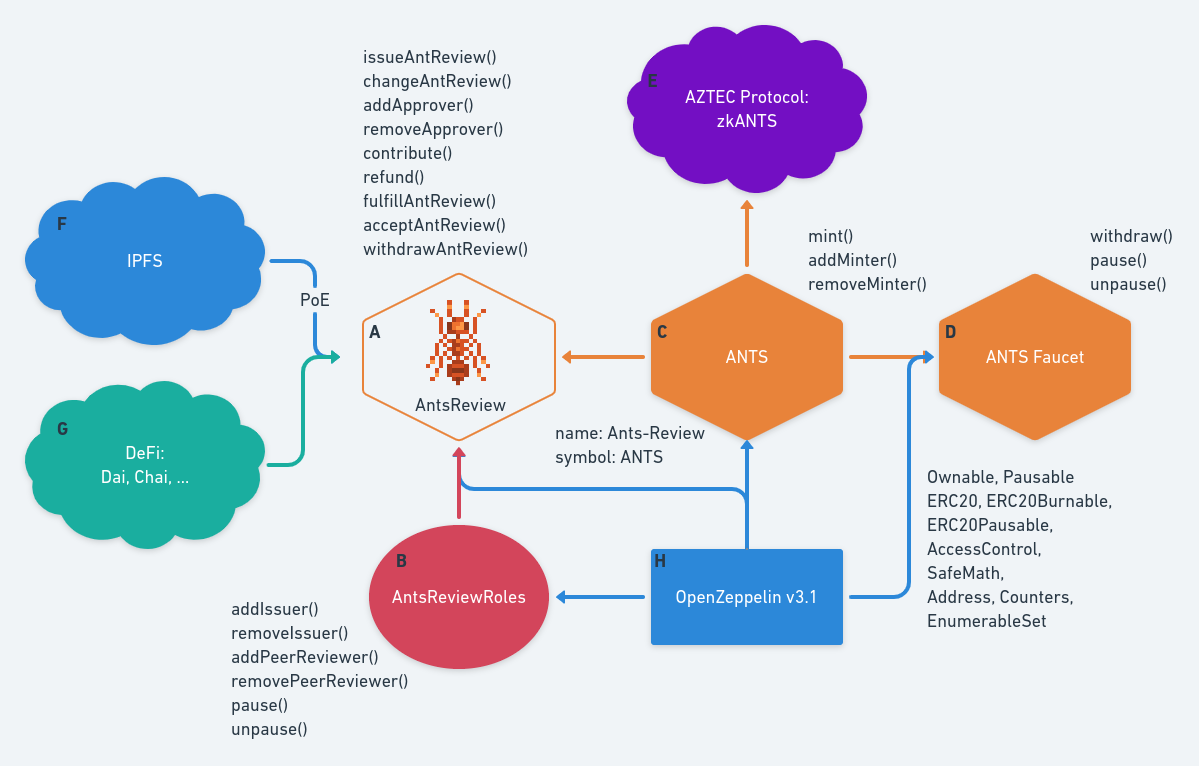
\includegraphics[scale=0.28]{Ants-Review}

\begin{enumerate}}
  \item \textbf{Bounty} - manage access management and the basic system.
  \item \textbf{Token Economics} - manage system incentivization mechanism integrating ideas from DeFi and Quadratic Funding.
  \item \textbf{Privacy} - mantains the anonymity of the system via AZTEC Protocol.
  \item \textbf{DAO} - manage the governance of the system via DemocracyDAO.
\end{enumerate}

\subsubsection{Bounty}


\begin{lstlisting}[language=Solidity]
pragma solidity 0.4.16;

contract TestContract {

	string private myString = "foo";

	function getString() constant returns (string) {
	    return myString;
	}

	function setString (string _string) {
	    myString = _string;
	}
}
\end{lstlisting}

\subsubsection{Token Economics}

\subsubsection{Quadratic Funding}

\subsubsection{Privacy}

\subsubsection{DAO}


\subsubsection{Future steps}
Future integrations that were not contemplated in the above presented PoC /demo but that we plan to cover for the development of the AntsReview bounty include: an ERC20 token, named Ant,  symbol ANT; Proof of Existence (PoE) service; memory storage on IPFS; moreover, since we wanted to anonymize peer-reviews to protect the contributors privacy, we would like to implement on the ANT token a fast, non-interactive type of zero-knowledge privacy protocol to enable private transactions on Ethereum. Zero-knowledge proof is a mathematical cryptographic method that through values permutations allows one party (the prover) to prove to another (the verifier) the veracity of a statement, without having to reveal what the statement is. We will use ZK-SNARKs (which stands for “Zero-Knowledge Succinct Non-Interactive Argument of Knowledge”) via the open source libraries of AZTEC protocol [15]. We will also use Ethereum Name Service (ENS) [14] to allow for human-readable Ethereum addresses; Upgradability Design Patterns [13] via Proxy, to allow the logic to be extended and improved; De-Fi integrations such as Dai, Chai. Finally, we would like to propose for AntsReview Quadratic Funding, a design written by Vitalik Buterin and co [20] and which applies concepts inspired by quadratic voting to funding public goods.

\section{Conclusion and Discussions}
In this whitepaper we addressed a central problem within the quality control academic dissemination: the peer-review process. We showed how blockchain technology could provide an efficient and viable solution and open up possibile directions for a change in paradigm in scientific communication. We proposed an incentive mechanism that could solve the problems of lack of acknowledgment and trust during peer-review. We exposed the architecture of our project and our Proof of Concept (PoC) for which we adopted cutting-edge tools from the open source blockchain community.

\section{Supplementary material}
Our open source code is available at the Github repository. A demo of the project is available at Youtube channel.
\section{CRediT Authorship Contribution Statement}
Bianca Trovò: Conceptualization, Investigation, Visualization, Writing - original draft, Writing - review \& editing. Nazzareno Massari: Project administration, Methodology, Validation, Software development. Both authors equally contributed and supervised the project.
\section{Declaration of Competing Interest}
The authors declare no competing interests.

% ---- Bibliography ----
%
% BibTeX users should specify bibliography style 'splncs04'.
% References will then be sorted and formatted in the correct style.
%
\bibliographystyle{splncs04}
\bibliography{references.bib}

\end{document}
